% !TEX TS-program = pdflatex
% !TEX encoding = UTF-8 Unicode

% This is a simple template for a LaTeX document using the "article" class.
% See "book", "report", "letter" for other types of document.

\documentclass[11pt]{article} % use larger type; default would be 10pt

\usepackage[utf8]{inputenc} % set input encoding (not needed with XeLaTeX)

%%% Examples of Article customizations
% These packages are optional, depending whether you want the features they provide.
% See the LaTeX Companion or other references for full information.

%%% PAGE DIMENSIONS
\usepackage{geometry} % to change the page dimensions
\geometry{a4paper} % or letterpaper (US) or a5paper or....
% \geometry{margins=2in} % for example, change the margins to 2 inches all round
% \geometry{landscape} % set up the page for landscape
%   read geometry.pdf for detailed page layout information

\usepackage{graphicx} % support the \includegraphics command and options

% \usepackage[parfill]{parskip} % Activate to begin paragraphs with an empty line rather than an indent

%%% PACKAGES
\usepackage{booktabs} % for much better looking tables
\usepackage{array} % for better arrays (eg matrices) in maths
\usepackage{paralist} % very flexible & customisable lists (eg. enumerate/itemize, etc.)
\usepackage{verbatim} % adds environment for commenting out blocks of text & for better verbatim
\usepackage{subfig} % make it possible to include more than one captioned figure/table in a single float
\usepackage{amsmath}
\usepackage{amsfonts}
\usepackage{amssymb}
\usepackage[normalem]{ulem}
\usepackage{listings}
\usepackage{mcode}
\usepackage{color}
\usepackage{bbm}
\usepackage{multirow}
\usepackage{rotating}
\usepackage{url}
\usepackage{hyperref}
\usepackage{float}
\restylefloat{table}
%\usepackage[it]{subfigure}


% These packages are all incorporated in the memoir class to one degree or another...

%%% HEADERS & FOOTERS
\usepackage{fancyhdr} % This should be set AFTER setting up the page geometry
\pagestyle{fancy} % options: empty , plain , fancy
\renewcommand{\headrulewidth}{0pt} % customise the layout...
\lhead{}\chead{}\rhead{}
\lfoot{}\cfoot{\thepage}\rfoot{}

%%% SECTION TITLE APPEARANCE
\usepackage{sectsty}
\allsectionsfont{\sffamily\mdseries\upshape} % (See the fntguide.pdf for font help)
% (This matches ConTeXt defaults)

%%% ToC (table of contents) APPEARANCE
\usepackage[nottoc,notlof,notlot]{tocbibind} % Put the bibliography in the ToC
\usepackage[titles,subfigure]{tocloft} % Alter the style of the Table of Contents
\renewcommand{\cftsecfont}{\rmfamily\mdseries\upshape}
\renewcommand{\cftsecpagefont}{\rmfamily\mdseries\upshape} % No bold!

\newcommand{\todo}{\textcolor{red}}

\DeclareMathOperator{\Tr}{Tr}
\DeclareMathOperator{\Hill}{Hill}
\DeclareMathOperator{\Dale}{Dale}
\newcommand{\grad}{\nabla}

\newcommand{\etc}{{\it etc}}
\newcommand{\eg}{{\it e.g.}}
\newcommand{\ie}{{\it i.e.}}
\newcommand{\wrt}{{\it w.r.t. }}
\newcommand{\etal}{{\it et al.}}

\newtheorem{theorem}{Theorem}
\newtheorem{lemma}{Lemma}
\newtheorem{axiom}{Axiom}
\newtheorem{assumption}{Assumption}
\newtheorem{principle}{Principle}
\newtheorem{result}{Result}
\newtheorem{corollary}{Corollary}
\newtheorem{notation}{Notation}
\newtheorem{definition}{Definition}
\newtheorem{prediction}{Prediction}
\newtheorem{proposition}{Proposition}
\newtheorem{example}{Example}
\newtheorem{observation}{Observation}
\newtheorem{remark}{Remark}
\newtheorem{question}{Question}

\definecolor{CriticalPoint}{RGB}{0, 127, 255}

%%% END Article customizations

%%% The "real" document content comes below...

\title{\textbf{Qualitative Representation of Images}}
\author{Firat Kalaycilar and Benjamin Kimia}
%\date{March 27, 2012} % Activate to display a given date or no date (if empty),
         % otherwise the current date is printed 

\begin{document}
\maketitle


\tableofcontents
\newpage

\section{TODO List}
\begin{enumerate}
\item \sout{Include experimental results (copy them from the tech report ppt)}
\item \sout{Add visual examples of the issues of the current implementation}
\item \sout{Algorithm correction: no need for Mask images, Label images are sufficient}
\item Integrate Prof. Kimia's comments
\item \sout{Add examples for each event pixel classification case}
\item Add more questions and answers
\item Clean up the code
\end{enumerate}

\newpage

\input{introduction}
\input{relatedwork}
\section{Theoretical Aspect}
\subsection{Terminology and Notation}
\label{sec:terminology}

\begin{table}[H]
\begin{center}    
    \begin{tabular}{ | c | c | c |}
    \hline
    \textbf{Concept} & \textbf{Definition} & \textbf{Notation}\\
    \hline
    Topographical surface  &  & $z = f(x,y)$\\
    \hline
    Gradient & $\grad f = [f_x, f_y]$ & $\grad f$ \\
    \hline
    Ortho-gradient & $\grad f^\perp = [-f_y, f_x]$ & $\grad f^\perp$\\
    \hline
    Hessian & $H = \left[ 
    	\begin{array}{cc}
	f_{xx} & f_{xy} \\
	f_{xy} & f_{yy} 
 	\end{array} \right]$& $H$ \\
    \hline
    Determinant of Hessian & $|H| = \det(H) = f_{xx}f_{yy} - f_{xy}^2$ & $|H|,\det(H)$\\
    \hline
    Trace of Hessian & $\Tr(H) = f_{xx} + f_{yy}$ & $\Tr(H)$\\
    \hline
    Laplacian & $\Delta f = f_{xx} + f_{yy} = f_{uu} + f_{vv}$ & $\Delta f$ \\
    \hline
    Eccentricity & $\varepsilon^2 = \frac{1}{4}(f_{xx} - f_{yy})^2 + f^2_{xy} $ & $\varepsilon$\\
    \hline
    Principal curvatures & Eigenvalues of $H$, $\Delta f \pm \varepsilon$ & $\lambda_1$, $\lambda_2$ \\
    \hline
    Principal curvature directions & Eigenvectors of $H$ & $e_1$, $e_2$ \\
    \hline
    Regular point & Non-critical point where $|\grad f| > 0 $& \\
    \hline
    Peak (Morse max) & $|\grad f| = 0$, $\det(H) > 0$, $\Tr(H) < 0$ & $\color{CriticalPoint}\boldsymbol{\bigtriangleup}$ \\
    \hline
    Pit (Morse min) & $|\grad f| = 0$, $\det(H) > 0$, $\Tr(H) > 0$ & $\color{CriticalPoint}\boldsymbol{\circ}$ \\
    \hline
    Pass/bar (Morse saddle) & $\grad f = 0$, $\det(H) < 0$ & $\color{CriticalPoint}\boldsymbol{+}$ \\
    \hline
    Degenerate critical point & $\det(H) = 0$ & \\
    \hline
    Level-set contour & $\beta(0) = P$, $\beta'(s) = -\grad f^\perp(\beta(s))/|\grad f^\perp(\beta(s))|$ & $\beta(s)$  \\
    \hline
    Slope line (integral curve) & $\alpha(0) = P$, $\alpha'(s) = -\grad f(\alpha(s))/|\grad f(\alpha(s))|$ & $\alpha(s)$  \\
    \hline
    Slope line segment & \shortstack{The slope line between two adjacent critical points.} & \\
    \hline
    Hill associated with peak $p_0$ &  \shortstack{$\{ p \;| \; \exists \text{ slope line segment through $p$ that ends at $p_0$}\}$} & $\Hill(p_0)$\\
    \hline
    Dale associated with pit $p_0$ & $\{ p \;| \; \exists \text{ slope line segment through $p$ that ends at $p_0$}\}$ & $\Dale(p_0)$\\
    \hline
    Watershed line & \shortstack{Dale boundaries. \\Special slope lines connecting saddles to peaks. \\According to Rothe/Reiger \cite{Rieger:IJCV97}, this definition \\ may not be true under degenerate cases.} & WS\\
    \hline
    Watercourse line & \shortstack{Hill boundaries. \\Special slope lines connecting saddles to pits. \\According to Rothe/Reiger \cite{Rieger:IJCV97}, this definition \\may not be true under degenerate cases.}& WC\\
    \hline
    Slope district & \shortstack{Non-empty intersection of a hill and a dale \cite{Nackman:PAMI84};\\ monotonic region.} & SD\\
    \hline
    \end{tabular}
    
\end{center}
\end{table}


\begin{notation}
The \textbf{gradient} and \textbf{Hessian} of a function $f(x,y)$ are denoted by $\grad f~=~[f_x, f_y]$ and $H = \left[ 
    	\begin{array}{cc}
	f_{xx} & f_{xy} \\
	f_{xy} & f_{yy} 
 	\end{array} \right]$.
\end{notation}

\begin{definition}
A \textbf{non-degenerate critical point} of a function $f(x,y)$ occur at points where $|\grad f| = 0$, and $|H_f| \neq 0$.
\end{definition}

\begin{notation}
Recall that the derivative of $f$ in the direction of the unit vector $T$ which is parametrized by variable $\xi$ is
\begin{equation*}
\frac{\partial f}{\partial \xi} = \grad f \cdot T.
\end{equation*}
\end{notation}

\subsection{Questions, Propositions and Proofs}

The slope line at each point can be obtained by integrating an ODE $\alpha'(s) = -\grad f(\alpha(s))$ where $\alpha(s)$ is the slope line.

\begin{proposition}
	 There is only one slope line through each regular point $P$ since the ODE, $\alpha'(s) = -\grad f(\alpha(s))$, with initial value for $\alpha(0) = P$ has a unique solution.	 
\end{proposition}
This is an explicit ODE for which there is a unique solution by the existense and uniqueness theorem \cite{Rieger:IJCV97}. Also see \cite{UniquenessTheoremWiki}.

\begin{proposition}
	The end points of a slope line segment, \ie, the slope line between two consecutive critical points, cannot both be a pit or both be a peak.
\end{proposition}
Let both $p_1$ and $p_2$ be two consecutive peaks on a slope line segment. Without loss of generality, assume that the downward flow is from $p_1$ to $p_2$. Since all slope lines around a peak must be outgoing, there is a contradiction in $p_2$ having an incoming slope line. Therefore, we can say that both end points cannot be a peak. A similar proof can be given for the pit case.

\begin{corollary}
	Can we have two slope lines meeting tangentially or intersecting transversely at a regular point?
\end{corollary}
No. Assume two slope lines meet at regular point $p$. Then, if we solve the slope line ODE with $\alpha(0) = p$, we should get two separate curves. But, we already know that the solution is unique, so that would be a contradiction.  

\begin{question}
	How do slope lines behave near min/max points?
\end{question}
\begin{figure}
\centering
\subfloat[max]{\label{fig:minslopelines}\includegraphics[height=.15\textheight]{img/max-slope-lines.png}}\;
\subfloat[min]{\label{fig:maxslopelines}\includegraphics[height=.15\textheight]{img/min-slope-lines.png}}
\subfloat[saddle]{\label{fig:saddleslopelines}\includegraphics[height=.15\textheight]{img/saddle-slope-lines.png}}\;
\caption{Slope line behaviour near critical points. $e_1$ and $e_2$ are the principal curvature directions. Figures were taken from \cite{Nackman:PAMI84}.}
\label{fig:cpslopelines}
\end{figure}
All slope lines approach mininima/maxima tangent to one of the principal curvatures \cite{Nackman:PAMI84}. See Figures \ref{fig:minslopelines} and \ref{fig:maxslopelines}. If the point is umbilical, the slope lines approach from all directions. This can be verified using a Monge patch. Let $f(x,y) = a x^2 + b y^2$ be the surface of interest where the signs of $a$ and $b$ are the same. Note that $(0,0)$ is either a max or a min point. Let $p_0 = (\epsilon \cos \theta, \epsilon \sin \theta)$ be a point on a slope line originating from $(0,0)$. Observe that as $\epsilon$ goes to $0$, the vector $p_0 - (0,0) = (\epsilon \cos \theta, \epsilon \sin \theta)$ becomes tangent to $\grad f(p_0) = (2 a \epsilon \cos \theta, 2 b \epsilon \sin \theta)$. This implies that $(2a \epsilon \cos \theta, 2b \epsilon \sin \theta) \cdot(\epsilon \sin \theta, - \epsilon \cos \theta) = 0$ which reduces to $(a-b) \sin 2\theta = 0$. If the point is not umbilical, $a \neq b$, then $\theta = 0$ or $\theta = \pi/2$ which are the pricincipal curvature directions. On the other hand, if $a = b$, the value of $\theta$ is arbitrary.

\begin{question}
	How do slope lines behave near saddle points?
\end{question}
See Figure \ref{fig:saddleslopelines}. We can use the same argument to show that the slope lines approach saddles along $e_1$ and $e_2$. Consider the Monge patch $f(x,y) = a x^2 + b y^2$ where $a$ and $b$ have opposite signs. Using the same approach we applied in the previous question, we obtain $(a-b) \sin 2\theta = 0$. In this case, it is guaranteed that $a \neq b$. Thus, $\theta = 0$ or $\theta = \pi/2$ are the solutions which correspond to the principle curvature directions. 
\begin{question}
	How do we characterize the hill corresponding to each peak?
\end{question}
Let $p_0$ be a peak. Then, $\Hill(p_0) = \{ p \;| \; \exists \text{ slope line segment through $p$ whose one end point is $p_0$}\}$. Similarly, if $p_0$ is a pit, $\Dale(p_0) = \{ p \;| \; \exists \text{ slope line segment through $p$ whose one end point is $p_0$}\}$.

\begin{question}
	Can two saddle points be connected with watershed/watercourse lines in generic images?
\end{question}
This can happen, but maybe an intrinsically unstable event \cite{Rosin:JVCIR95}, so it may not be generic. We have experience that saddle-saddle connections act like a watershed and watercourse line at the same time.
\begin{question}
	Can hills/dales be multiply connected?
\end{question}
No. Suppose we have a hill with two disconnected regions. The points in the region without the peak must be connected to the peak with slope lines by definition. Since a region cannot be disconnected from a region containing the peak and have slope lines connected to the peak at the same time, we can say that hills cannot be composed of disconnected regions. \todo{[pathwise connectivity]}

\begin{question}
	Do hills partition the image domain completely? In other words, is there any point in the domain that does not belong to any hill?
\end{question}
Every image point either belongs to a hill (corresponding to a peak) or to a watercourse line (which separates two hills).
%There is a slope line for every regular point. If we follow slope lines in the upward flow direction starting at a regular point $p$, we will reach a critical point which is either a peak or a saddle. If it is a peak, then $p$ belongs to the associated hill. But if it is a saddle, then $p$ belongs to a watercourse line. Therefore, the points other than those belonging to watercourse lines belong to hills.
Similarly,  every image point belongs to a dale (which corresponds to a pit) or to a watershed line (which separates two dales).
\begin{proposition}
	Hills are tightly surrounded by watercourse lines. In other words, watercourse lines correspond to hill boundaries. 
\end{proposition}
Yes. \todo{Don't know how to prove this!}

\begin{figure}
\centering
\includegraphics[width=.45\textwidth]{img/slope-district-catalog.png}
\caption{Catalog of slope districts. Taken from \cite{Nackman:PAMI84}.}
\label{fig:slopedistrictcatalog}
\end{figure}

\begin{question}
	Are saddle-saddle connections possible?
\end{question}
Yes. See Nackman's slope district catalog \cite{Nackman:PAMI84}. (Figure \ref{fig:slopedistrictcatalog}). It is not clear whether watershed, watercourse or both simultaneously connect them.
\begin{question}
	Are saddle-saddle connections generic?
\end{question}
\todo{TODO}
\begin{question}
	Is there any critical point that does not belong to a watershed/watercourse line?
\end{question}
No. There are slope line segments going in or out of each critical point. And those segments always have another end point (possibly out of boundaries in the case of images) which is also a critical point. Based on the type of the end points, these slope line segments are either watershed or watercourse lines.
\begin{question}
	Can there be any watershed/watercourse line without any critical points?
\end{question}
No. Watershed/watercourse lines are slope line segments, so by definition their end points are always critical points.
\begin{proposition}
	There is no other max point on a hill boundary.
\end{proposition}
Assume that $p$ is a max point on the boundary of hill $h$. In some neighborhood of $p$ with no other critical points, all the upward flowing slope lines converge to $p$. Since this neighborhood intersects $h$, all the points in the intersection must belong to $h$ and the hill corresponding to $p$ at the same time. Since this is not possible, we can say that there cannot be any peaks on a hill boundary.

\noindent Another explanation: Hill boundaries are composed of watercourse lines, so there can only be regular, min and saddle points. 
\begin{proposition}
	There is at least one saddle and one min (max) point on a hill (dale) boundary.
\end{proposition}
\todo{[This proof ignores the saddle-saddle connections. INCORRECT.]} Since hills are bounded by watercourse lines whose end points are always a min and a saddle point, it is clear that there must be at least one min and one saddle point on a hill boundary.

\begin{proposition}
	Saddles and min points are arranged in an alternating pattern on a hill boundary.
\end{proposition}
\todo{[Probably INCORRECT]} Since there is no slope line with min-min or saddle-saddle end points, min and saddle points must be in an alternating pattern.
\begin{proposition}
The number of saddles and min points is the same on a hill boundary.
\end{proposition}
\todo{[Probably INCORRECT]} The closed alternating pattern guarantees that the number of saddles and min points is the same.
\begin{question}
	Can there be another critical point inside a hill (dale) other than the associated peak (pit)?
\end{question}
\todo{There is an example showing a special case in \cite{Bremer:etal:TVCG04} on page 3. A min and a saddle point are inside the centeral hill. This example is important, because it is generic and might affect our definition of slope districts.}
\begin{corollary}
Slope lines from a hill (dale) meet the hill boundary transversely at a saddle and tangentially at a min.
\end{corollary}
Figure \ref{fig:cpslopelines} gives an idea about why this should be correct. Observe how slope lines meet the critical points.

\subsection{Ridge and Valley Topographic Curves}
\begin{definition} 
A {\em ridge} or {\em valley} point of $z=f(x,y)$ is a point where
\begin{equation}
\overrightarrow{\grad f}.\overrightarrow{\nu_1} = 0, \label{eq:07-27-06:starstar10}
\end{equation}
where $\nu_1$ is the eigenvector with the largest eigenvalue of the Hessian of $f$, and where the
eigenvalue $\lambda_1>0$ or $\lambda_1<0$, respectively. \todo{[Letting $\xi$ parametrize direction $\overrightarrow{\nu}$, we have]}
\end{definition}

\noindent In analogy to the condition in 1D used to distinguish minima from maxima among the extrema of 1D functions, namely,
whether $f^{''}(x)$ is positive or negative, respectively, ridges and valleys are distinguished using the
second derivative in the direction $\nu_1$,
\begin{equation*}
\frac{\partial^2 f}{\partial\xi^2} = \nu_1^T H \nu_1 
= \nu_1^T(\lambda_1 \nu_1)
= \lambda_1,
\end{equation*}
which gives just the eigenvalue $\lambda_1$.
Thus, if $\lambda_1 < 0$, we have a ridge and if $\lambda_1 > 0$ we have a valley. The case $\lambda_1=0$ also implies $\lambda_2=0$
since $\lambda_1$ is the larger eigenvalue. In such a case higher-order derivatives needs to be consulted to determine a ridge.


\section{Computing Critical Points and Their Connectivity}

This section presents two important algorithms required to compute the critical points of an image and their connectivity. The first algorithm detects both the minima and watershed pixels and is called $min\_watershed\_detector(I, \sigma)$ where $I$ is the image and $\sigma$ is a smoothing parameter. Note that the same function can be used to detect maxima and watercourse by inverting the image. Its implementation is very similar to the standard watershed transform which works as follows \cite{WatershedWiki}: A set of seed pixels is selected and given different labels. The pixels surrounding the seed pixels are inserted into a priority queue where the pixel priority is based on how low its intensity value is. Then, the pixel with highest priority is chosen. If its already labeled neighbors have the same label, it is given that label. Otherwise, it is kept unlabeled. Then, all unlabeled neighboring pixels are added to the priority queue. The algorithm goes on like this until the priority queue becomes empty. At the end, the labeled pixels are the basins while the unlabeled ones correspond to watershed pixels. The key differences of our algorithm from the traditional one are: \textit{(i)} There is no need for an apriori detection of minima (the seed pixels) since the detection is an integral part of the algorithm; \textit{(ii)} The algorithm keeps track of the identities of the minima giving rise to each watershed pixel. 
Note that $min\_watershed\_detector(I, \sigma)$ may also be implemented  by separating the detection of extended minima\footnote{An extended minima is a connected cluster of pixels with the same intensity value surrounded by higher intensity pixels. An implementation of this is MATLAB's $imregionalmin$.} as a first, separate stage, and then using the traditional watershed transform to label pixels either as the watershed pixels or basins. Next, using the basin labels that are neighbors to each watershed pixel, the identities of the minima giving rise to each watershed pixel can be found\footnote{Not sure if this would be identical to what we compute in our algorithm.}.

The second algorithm, $TAG\_detector(I, \sigma)$, aims to find saddles and then connect all the critical points, namely, minima, maxima and saddle points in a graph structure called Topological Appearance Graph (TAG). It uses the minima and watershed pixels detected by the $min\_watershed\_detector(I, \sigma)$ and the maxima and watercourse pixels detcted by the $min\_watershed\_detector(-I, \sigma)$. Since our definition of saddles is the intersection of watershed and watercourse lines, it utilizes the watershed/watercourse pixels to localize the saddles. In addition, since the ids of minima/maxima giving rise to watershed/watercourse pixels are known, the algorithm is able to establish connections between all the critical points which results in the TAG of the input image $I$. 
\\

\begin{figure}
\centering
\includegraphics[width=.45\textwidth]{img/self-collision.png}
\caption{A self-colliding basin. This case is currently ignored by the algorithm.}
\label{fig:selfcollision}
\end{figure}

\noindent \textbf{function $min\_watershed\_detector(I, \sigma)$:}
\\

\textbf{Summary:} The goal is to find all the minima and watershed pixels with the ids of the basins (minima) who gave rise to them. In order to achieve this, the intensity values in the image are first sorted from low to high. As in the traditional watershed transform, the intensity is thought of as rising water levels. Then, we visit each water level in increasing order and find out which pixels have just been covered with water (we call them \textit{event pixels}). Next, we classify each connected component of the event pixels in one of three classes: \textit{(i)} minimum, \textit{(ii)} watershed pixel or \textit{(iii)} basin growth (all pixels of a connected component are given the same label\footnote{Prof. Kimia asked me if it is possible to assign the pixels of a connected component to different classes. For example, can some part of the connected component be a basin growth while the other parts are watershed pixels? I do not know the answer. \todo{We need an explanation.}}). Note that if the connected component has more than one pixel, the result is an \textit{extended} minimum, \textit{extended} watershed or \textit{extended} basin growth. Once all the water levels are visited, the algorithm stops. For the detailed algorithm steps, see below:
\\

\textbf{Failure mode:} Self-collisions are not handled (Figure \ref{fig:selfcollision}). Some watershed pixels may not be detected which will cause the algorithm to miss the saddles due to self-collisions. 
\\

\noindent \textbf{Input:} 
\begin{itemize}
\item Image $I$
\item $\sigma$ for smoothing
\end{itemize}

\noindent \textbf{Output:} 
\begin{itemize}
\item $ws$: the unorganized list of watershed pixels
\item $mins$: the minima of $I$
\item $ws\_basins$: ids of the minima giving rise to each watershed pixel
\end{itemize}
\textbf{Local variables:}
\begin{itemize}
\item $i$: the index of the loop visiting the sorted water levels.
\item $sorted\_I$: the sorted array of unique intensity values in $I$.
\item $Water\_Level$: the level of the rising water.
\item $Label\_prev$: an image with the same size as $I$. Each pixel holds the basin id assigned to it before visiting the current water level. 0 means ``not assigned" yet.
\item $Label\_curr$: an image with the same size as $I$. Each pixel holds the basin id assigned to it after visiting the current water level. 0 means ``not assigned" yet.
\item $num\_min$: the number of minima.

\end{itemize}

\begin{figure}
\centering
\includegraphics[width=.85\textwidth]{img/boundary.png}
\caption{In this example, the blue triangles are the maxima, the blue circles are the minima, the red x's are the watershed, the green x's are the watercourse and the yellow x's are the intersection of the watershed and watercourse pixels. Observe the image boundary pixels after processing the image with mirror reflection padding. Most of the boundary pixels are either critical points or watershed/watercourse pixels. The only exception happens when there is a direct transition from a minimum to maximum along the boundary.}
\label{fig:reflectionboundary}
\end{figure}

\begin{figure}
\centering
\subfloat[Watershed creation. Since the event pixel is adjacent to two separate basins, it is classified as a watershed pixel.]{\label{fig:wscreation}\includegraphics[height=.25\textheight]{img/eventpix/watershedcreation.png}}\;
\subfloat[Watershed growth. The orange pixels are the previously classified watershed pixels and the red, green, cyan and yellow regions correspond to 4 seperate basins. Since the event pixel is only adjacent to the existing watershed pixels, it is classified as a watershed pixel as well.]{\label{fig:wsgrowth}\includegraphics[height=.25\textheight]{img/eventpix/watershedgrowth.png}}\\
\subfloat[Basin creation. Since the event pixel is not adjacent to any watershed or basin pixel, it is classified as a new basin (minimum).]{\label{fig:basincreation}\includegraphics[height=.25\textheight]{img/eventpix/basincreation.png}}\;
\subfloat[Basin growth. Since the event pixel is adjacent to only one basin, it is just a part of that basin. Thus, it is classified as a basin pixel.]{\label{fig:basingrowth}\includegraphics[height=.25\textheight]{img/eventpix/basingrowth.png}}
\caption{Event pixel classification examples. The white pixels are the event pixels to be classified.}
\label{fig:eventpixclasses}
\end{figure}

\textbf{Algorithm:}
\begin{enumerate}
	\item Pad the image boundary using the mirror reflection of the image. I use $(7\sigma-1)/2$ pixels for padding each side. The motivation for using mirror reflection instead of constant value continuation is that mirror reflection causes most of the boundary pixels to become either critical points or watershed/watercourse pixels. This is violated only when there is a direct transition from a minimum to maximum along the boundary, \ie the absence of a saddle point on the boundary to form a watershed/watercourse line. See Figure \ref{fig:reflectionboundary}.

	\item Smooth the padded image with a Gaussian with standard deviation $\sigma$. \footnote{This step may not be required in the future, as structural smoothing after graph construction may be more meaningful.}

	\item Sort all the intensity values in the image in ascending order to create $sorted\_I$.
	\item Start a loop with $i = 1$, $Label\_prev$ = initially all 0's and $num\_min = 0$ 
	\begin{enumerate}[i.]
		\item Set $Water\_Level$ = $sorted\_I[i]$.
		\item Compute the mask $Mask\_curr$: If the image intensity $\leq Water\_Level$, the mask is set to $-1$. Otherwise, it is set $0$. The reason for using $-1$ instead of $1$ will become clear shortly.
		\item $Label\_curr = Mask\_curr$.
		\item Copy non-zero labels from the previous iteration ($Label\_prev$) into $Label\_curr$. So, now $Label\_curr$ has the same labels as $Label\_prev$, but additionally it also has pixels labeled as $-1$ which correspond to new pixels covered with water, the so-called ``event pixels" which will correspond to either minima creation, watershed creation or basin growth.
		\item Classify each connected component of event pixels as ``min", ``watershed" or ``basin growth".
		\begin{enumerate}[(a)]
			\item \textbf{[watershed creation]} Figure \ref{fig:wscreation}. It is a ``watershed" if it touches at least 2 separate regions with non-zero labels. Add each pixel of the component to $ws$. Add the ids of the basins participating in the collision to $ws\_basins$. In this way, we always know which minima give rise to which watershed pixels.	
			\begin{enumerate}
				\item \textbf{[watershed growth]} Figure \ref{fig:wsgrowth}. \todo{Added this condition recently, not sure about its correctness.} It is a ``watershed" if it is surrounded by 0s in $Label\_curr$, but at least one of the surrounding pixels has been labeled as ``watershed". This case does not happen frequently, but it can still happen. However, I am not sure if this is the best way to handle it. In order to handle this case more properly, the watershed pixels can be represented as $-2$ in $Label\_curr$ and $Label\_prev$.
			\end{enumerate}		

			\item \textbf{[basin creation]} Figure \ref{fig:basincreation}. It is a ``min" if it is surrounded by 0s in $Label\_curr$ and none of the surrounding pixels has been labeled as ``watershed". Either fit a surface to find the subpixel position or take the centroid of the component and add it to $mins$. $num\_min = num\_min + 1$.		
			

			\item \textbf{[basin growth]} Figure \ref{fig:basingrowth}. It is a ``basin growth" if it touches only one region with a non-zero label. 
		\end{enumerate}
		
		\item Update $-1$s in $Label\_curr$ with appropriate labels (use label $-2$ for watershed creation, label $num\_min$ for basin creation and the label of the growing basin for basin growth)

		\item $Label\_prev = Label\_curr$.

		\item $i = i + 1$.
		
		\item Exit the loop if all the water-levels have been visited.
	\end{enumerate}
	5) Return $mins$, $ws$ and $ws\_basins$.\\\\
\end{enumerate}



\noindent \textbf{function $TAG\_detector(I, \sigma)$:}
\\

\textbf{Summary:} The graph connecting the critical points can only connect saddles to other critical points, \ie, the only connection of maximum and minimum is to saddle point and not to other maximum or minimum. So, we first compute the minima/maxima and watershed/watercourse pixels. Then, based on our definition of saddles, we intersect the watershed and watercourse pixels and find the saddle candidates. Next, we classify each candidate either as saddle or as a series of saddle points connected as a chain. Finally, we connect all the saddle points to minima, maxima and other saddles based on the identities of minima/maxima giving rise to each watershed pixel. This generates the TAG of $I$. 
\\

\textbf{Failure mode:} I do not have a generalized rule to find saddle-saddle connections. So, the saddle-saddle connections are ignored which causes the algorithm to create incorrect links in the TAG. \todo{Show examples.}
\\

\noindent \textbf{Input:} 
\begin{itemize}
\item Image $I$
\item $\sigma$ for smoothing
\end{itemize}

\noindent \textbf{Output:}
\begin{itemize}
\item $mins$: the list of minima of $I$
\item $maxs$: the list of maxima of $I$
\item $saddles$: the list of saddle points of $I$
\item $saddle\_links$: the ids of the minima/maxima/saddle points connected to each saddle. It corresponds to the TAG of $I$.
\end{itemize}

\noindent \textbf{Local variables:}
\begin{itemize}
\item $ws$: the unorganized list of watershed pixels of $I$
\item $wc$: the unorganized list of watercourse pixels of $I$
\item $ws\_basins$: ids of the minima giving rise to each watershed pixel
\item $wc\_hills$: ids of the maxima giving rise to each watercourse pixel
\item $ws\_wc\_common$: common pixels of $ws$ and $wc$
\item $saddle\_candidates$: the list of connected components in $ws\_wc\_common$
\end{itemize}

\begin{figure}
\centering
\subfloat[]{\includegraphics[height=.32\textheight]{img/connsaddle1.png}}\;
\subfloat[]{\includegraphics[height=.32\textheight]{img/connsaddle5.png}}\\
\subfloat[]{\includegraphics[height=.24\textheight]{img/connsaddle3.png}}\;
\subfloat[]{\includegraphics[height=.24\textheight]{img/connsaddle6.png}}\\
\subfloat[]{\label{fig:saddlecandidates}\includegraphics[width=.95\textwidth]{img/connsaddle4.png}}
\caption{In these examples, the blue triangles are the maxima, the blue circles are the minima, the red x's are the watershed, the green x's are the watercourse and the yellow x's are the intersection of the watershed and watercourse pixels. The yellow chains are the examples of the cases where I think the saddle-saddle connections occur. Note that there are other yellow groups with 1 or 2 pixels, too. Those are the examples of isolated saddle points. Do not confuse them with the saddle chains.}
\label{fig:connsaddle}
\end{figure}

\noindent \textbf{Algorithm:}
\begin{enumerate}
	\item Call $min\_watershed\_detector(I, \sigma)$  to compute $ws$, $mins$ and $ws\_basins$ 

	\item Call $min\_watershed\_detector(-I, \sigma)$ to compute $wc$, $maxs$ and $wc\_hills$ 

	\item Find the intersection of $ws$ and $wc$ and store these pixels in $ws\_wc\_common$. These are saddle points either as isolated saddle points or as chains of saddle points (See Figure \ref{fig:saddlecandidates}). Keep track of the ids in $ws\_basins$ and $wc\_hills$ and associate them with each pixel in $ws\_wc\_common$.

	\item Find the connected components in $ws\_wc\_common$ and store them in $saddle\_candidates$. 

	\item Classify and store each connected component in $saddle\_candidates$ as follows:
	\begin{enumerate}[i.]
		\item \label{item:regularsaddle} If all the pixels of the component have the same min and max ids according to their entries in $ws\_basins$ and $wc\_hills$, fit a quadratic surface to the entire component, find its subpixel critical point and add it to $saddles$. \footnote{Subpixel computation part is disabled, but there is code to accomplish that. For now, I just average the coordinates of the pixels that belong to the component.} 
		\item \label{item:connsaddle} Otherwise, this may imply that this component corresponds to at least two saddle points connected by saddle-saddle links. \footnote{I haven't been able to generalize this case, so it does not work for now.} See Figure \ref{fig:connsaddle} for examples of this case.
	\end{enumerate}

	\item Compute $saddle\_links$ (ids of minima/maxima/saddle points connected to each saddle) based on the component classification results. Basically, use the entries in $ws\_basins$ and $wc\_hills$ if it is classified according to Step \ref{item:regularsaddle}. \todo{Use the connected saddle information if it is classified according to Step \ref{item:connsaddle}.}

	\item Return $mins$, $maxs$, $saddles$ and $saddle\_links$. 
\end{enumerate}




\input{experiments}
\section{Future Directions}
\subsection{Local TAG structures as feature descriptors}
As shown in Section \ref{sec:experiments}, critical points are promising interest points. In our experiments, we treated each critical point as a standalone interest point represented by a SIFT descriptor. However, there exists a more natural way to describe critical points: TAG.

\begin{figure}
\centering
\subfloat[]{\includegraphics[height=.18\textheight]{img/localtag/loctag1.png}}\;
\subfloat[]{\includegraphics[height=.18\textheight]{img/localtag/loctag2.png}}\;
\subfloat[]{\includegraphics[height=.18\textheight]{img/localtag/loctag3.png}}\;
\subfloat[]{\includegraphics[height=.18\textheight]{img/localtag/loctag4.png}}
\caption{Local TAG structures. These graphs can be used to describe the critical points.}
\label{fig:loctag}
\end{figure}

TAG captures the local neighborhood structure of critical points which seems to be a distinctive representation. See Figure \ref{fig:loctag} for examples of local TAG structures. Our idea for computing the dissimilarity of two critical points is as follows: Given two local TAG structures, we plan to apply certain graph edit operations to convert one of the graphs to the other. The resulting edit distance can then be used as a matching score or dissimilarity. Some possible graph edits are
\begin{itemize}
\item Global transformations (rotation and scaling)
\item Edge deletion
\item Individual edge rotation
\item Individual edge scaling
\item Intensity change
\item Curvature change.
\end{itemize}

\subsection{Level-set implementation}
The current algorithm is processing the water levels using a discrete process which has its own problems. For example (see Figure \ref{fig:saddlecandidates}), in our discrete process, the watershed (or watercourse) lines sometimes form junctions without any critical points. It does not make any sense, since there must pass only one slope line from a regular point. Prof. Kimia believes that this kind of artifacts due to discreteness might be avoided in a level-set framework. 

The proposed idea is to visit the water levels by evolving a level-set function according to the underlying intensity values. Prof. Kimia believes that their paper on ``shape form shading" \cite{Kimmel:Shape:Shading} has a similar level-set formulation. 

\subsection{Organizing the watershed/watercourse pixels}

The current algorithm produces a set of unorganized watershed and watercourse pixels. However, organizing them as curves might help understand some of the problems we are facing (\eg, the watershed junctions making no sense). In addition, it will be useful in getting the subpixel watershed lines.   

\subsection{Image generation}

We had explored the possibility of generating images from given TAGs. Our method for image generation was fixing the intensity values at certain pixels and running the diffusion equation on the image. See the examples in Figure \ref{fig:imagegeneration}.   


\begin{figure}
\centering
\subfloat[Fixed values at minima and maxima.]{\includegraphics[width=.95\textwidth]{img/max-min-generation.png}}\\
\subfloat[Fixed values at minima, maxima and saddles.]{\includegraphics[width=.95\textwidth]{img/max-min-saddle-generation.png}}\\
\subfloat[Fixed values at watershed and watercourse pixels.]{\includegraphics[width=.95\textwidth]{img/wswc-generation}}
\caption{Image generation with diffusion.}
\label{fig:imagegeneration}
\end{figure}

\pagebreak
\section{Appendix}

\begin{proposition}
	The curvatures of a slope line and a level set contour are
	\begin{equation*}
\kappa_\alpha = -\frac{(f_x^2-f_y^2) + f_x f_y (f_{yy}-f_{xx})}{(f_x^2 + f_y^2)^{\frac{3}{2}}},
\end{equation*}
\begin{equation*}
\kappa_\beta = \frac{f_y^2 f_{xx} - 2 f_x f_y f_{xy} + f_x^2 f_{yy}}{(f_x^2 + f_y^2)^{\frac{3}{2}}},
\end{equation*}
respectively.
\end{proposition}


\noindent Let $f(x,y) = c_0$, where $c_0$ is a constant be a level set curve of $\beta$ of $f$. Then, by differentiating this with respect
to arclength $\tilde s$ along $\beta$, we have
\begin{equation*}
\grad f . T_\beta = 0,
\end{equation*}
so that $T_\beta = \frac{\grad f^\perp}{|\grad f|}$. Differentiating again we have
\begin{equation*}
\frac{(\grad f^\perp)^T}{|\grad f|} H T_\beta + \grad f(\kappa_\beta N_\beta) = 0,
\end{equation*}
from which $\kappa$ can be obtained using $N_\beta=\frac{-\grad f}{|\grad f|}$ as
\begin{equation}
\kappa_\beta = \frac{\frac{1}{|\grad f|^2}(\grad f^\perp)^T H \grad f^\perp}{\grad f \frac{\grad f}{|\grad f|}} = \frac{f_y^2 f_{xx} - 2 f_x f_y f_{xy} + f_x^2 f_{yy}}{(f_x^2 + f_y^2)^{\frac{3}{2}}}. 
\end{equation}
The contour line curvature can also be expressed in $(u,v)$ coordinates as
\begin{equation}
\kappa_\beta = \frac{f_{vv}}{f_u}. \label{eq:08-08-06:star2}
\end{equation}

\noindent Similarly, for a slope line, the tangent $T_\alpha = \frac{\grad f}{|\grad f|}$ and
$N_\alpha = \frac{\grad f^T}{|\grad f|}$ we have

\begin{equation*}
\grad f^\perp.T_\alpha = 0.
\end{equation*}

\noindent Differentiating this with respect to arclength along $\alpha$ we have

\begin{equation*}
\frac{(\grad f^\perp)^T H}{|\grad f|} T_\alpha + \grad f^\perp (\kappa N_\alpha) = 0
\end{equation*}

\noindent from which $\kappa$ can be determined as

\begin{equation}
\kappa_\alpha = -\frac{\frac{(\grad f^\perp)^T H \grad f}{|\grad f|^2}}{\grad f^\perp \frac{\grad f^\perp}{|\grad f|}} 
= -\frac{(f_x^2-f_y^2) + f_x f_y (f_{yy}-f_{xx})}{(f_x^2 + f_y^2)^{\frac{3}{2}}}.
\end{equation}

\noindent This can also be written as

\begin{equation}
\kappa_\alpha = -\frac{f_{uv}}{f_u} \label{eq:11-06-06:star3}.
\end{equation}



\pagebreak
\bibliographystyle{plain}
\bibliography{paper,Kimia,vision,edge,medical,multiview,recognition,categorization,ridge,indexing,metric,nn-search,segmentation,deformable,url,perceptual-grouping,shape-papers,shape-matching,skeleton2D,texture,shape-from-shading,psychophysics,multidimscaling,surface-networks,proceedings}
\end{document}


%\paragraph{Proof:} We can use MATLAB for this proof:
%{\small
%\lstset{frame=shadowbox}
%\lstinputlisting{matlab_proof.m}}
%Since MATLAB's symbolic toolbox returns $(0,0)$ for all 3 cases, we can say that our proposition is correct.
